\chapter{Initial configuration}
\label{ch:initial_conf}
\section{Identification of sensor's axes}
\indent The first step that needs to be carried out is to determine the orientation of the axes of the body frame that we wish to use, as well as the orientation of the rotation around those axes. One of the most popular configurations is to set the X axis pointing forwards, the Y axis pointing to the right and the Z axis pointing down. This configuration follows the rule of the right hand for the orientation of the axes and the corkscrew rule for the rotation. Both are shown in Figure \ref{fig:bodyAxes}. These two standard navigation frames are usually employed when representing the orientation of a body in space and are known as the North-East-Down (NED) and the East-North-Up (ENU) frames.

\begin{figure}[H]
\centering
\includegraphics[width=0.6\textwidth]{figures/bodyAxes}
\caption{Definition of the desired body axes (a). Convention for the orientation of the axis rotation (b).}
\label{fig:bodyAxes}
\end{figure}
Since we will be using the GaitWatch device to monitor gait, then we need its X axis to point to the front of the patient, the Y axis pointing to the right of the patient, and the Z axis to the floor. We will start by configuring the orientation of the sensors which are inside the data gathering unit and which will be placed on the back of the patient. Figure \ref{fig:gwBox} shows the desired orientation for Gaitwatch's box.

\begin{figure}[H]
\centering
\includegraphics[width=0.6\textwidth]{figures/bodyAxesGW}
\caption{Orientation and axes of the GaitWatch box.}
\label{fig:gwBox}
\end{figure}

Once we know the desired orientation, the next step is to adapt the axes of the sensors' boards to it. We will start by adjusting the accelerometer. 

\subsection{Identification of Accelerometer's axes}
\label{subsec:acc_ID}

\indent The goal here is to determine the orientation of the axes and adapt it to the convention aforementioned. First, we set the box with the desired Z axis pointing downwards and upwards respectively while gathering data, as shown in figure \ref{fig:AccZaxis}.

Now we plot the acceleration gathered along the three axes. We have to identify the channel showing a large change in the measured acceleration.

\begin{figure}[H]
\centering
\includegraphics[width=0.6\textwidth]{figures/AccZaxis.jpg}
\caption{Identification of Z axis of the accelerometer in the box unit.}
\label{fig:AccZaxis}
\end{figure}
 
That channel will then be labeled as Z irrespective to which label it may have in the accelerometer board. That is, the sensor board may indicate that the selected channel is 'X' in the sensor frame, but we will label it as 'Z' in our desired frame which is the body frame. 

If the Z axis of the sensors has the same orientation of the desired frame, then, when pointing the Z axis of the box downwards, the accelerometer will measure 1g since its axis is parallel to the Earth's gravity vector. If it has the opposite orientation, then the accelerometer will measure -1g. Since we have not calibrated the accelerometer so far and, therefore, the data are in raw units, the way to identify the correct orientation is by knowing that the measured output when setting the accelerometer axis parallel to gravity is larger than its output when it is set anti-parallel to the gravity vector. Figure \ref{fig:ZaxisAccSignals} shows the triaxial gathered acceleration and the axis which should be labeled as 'Z'.

\begin{figure}[H]
\centering
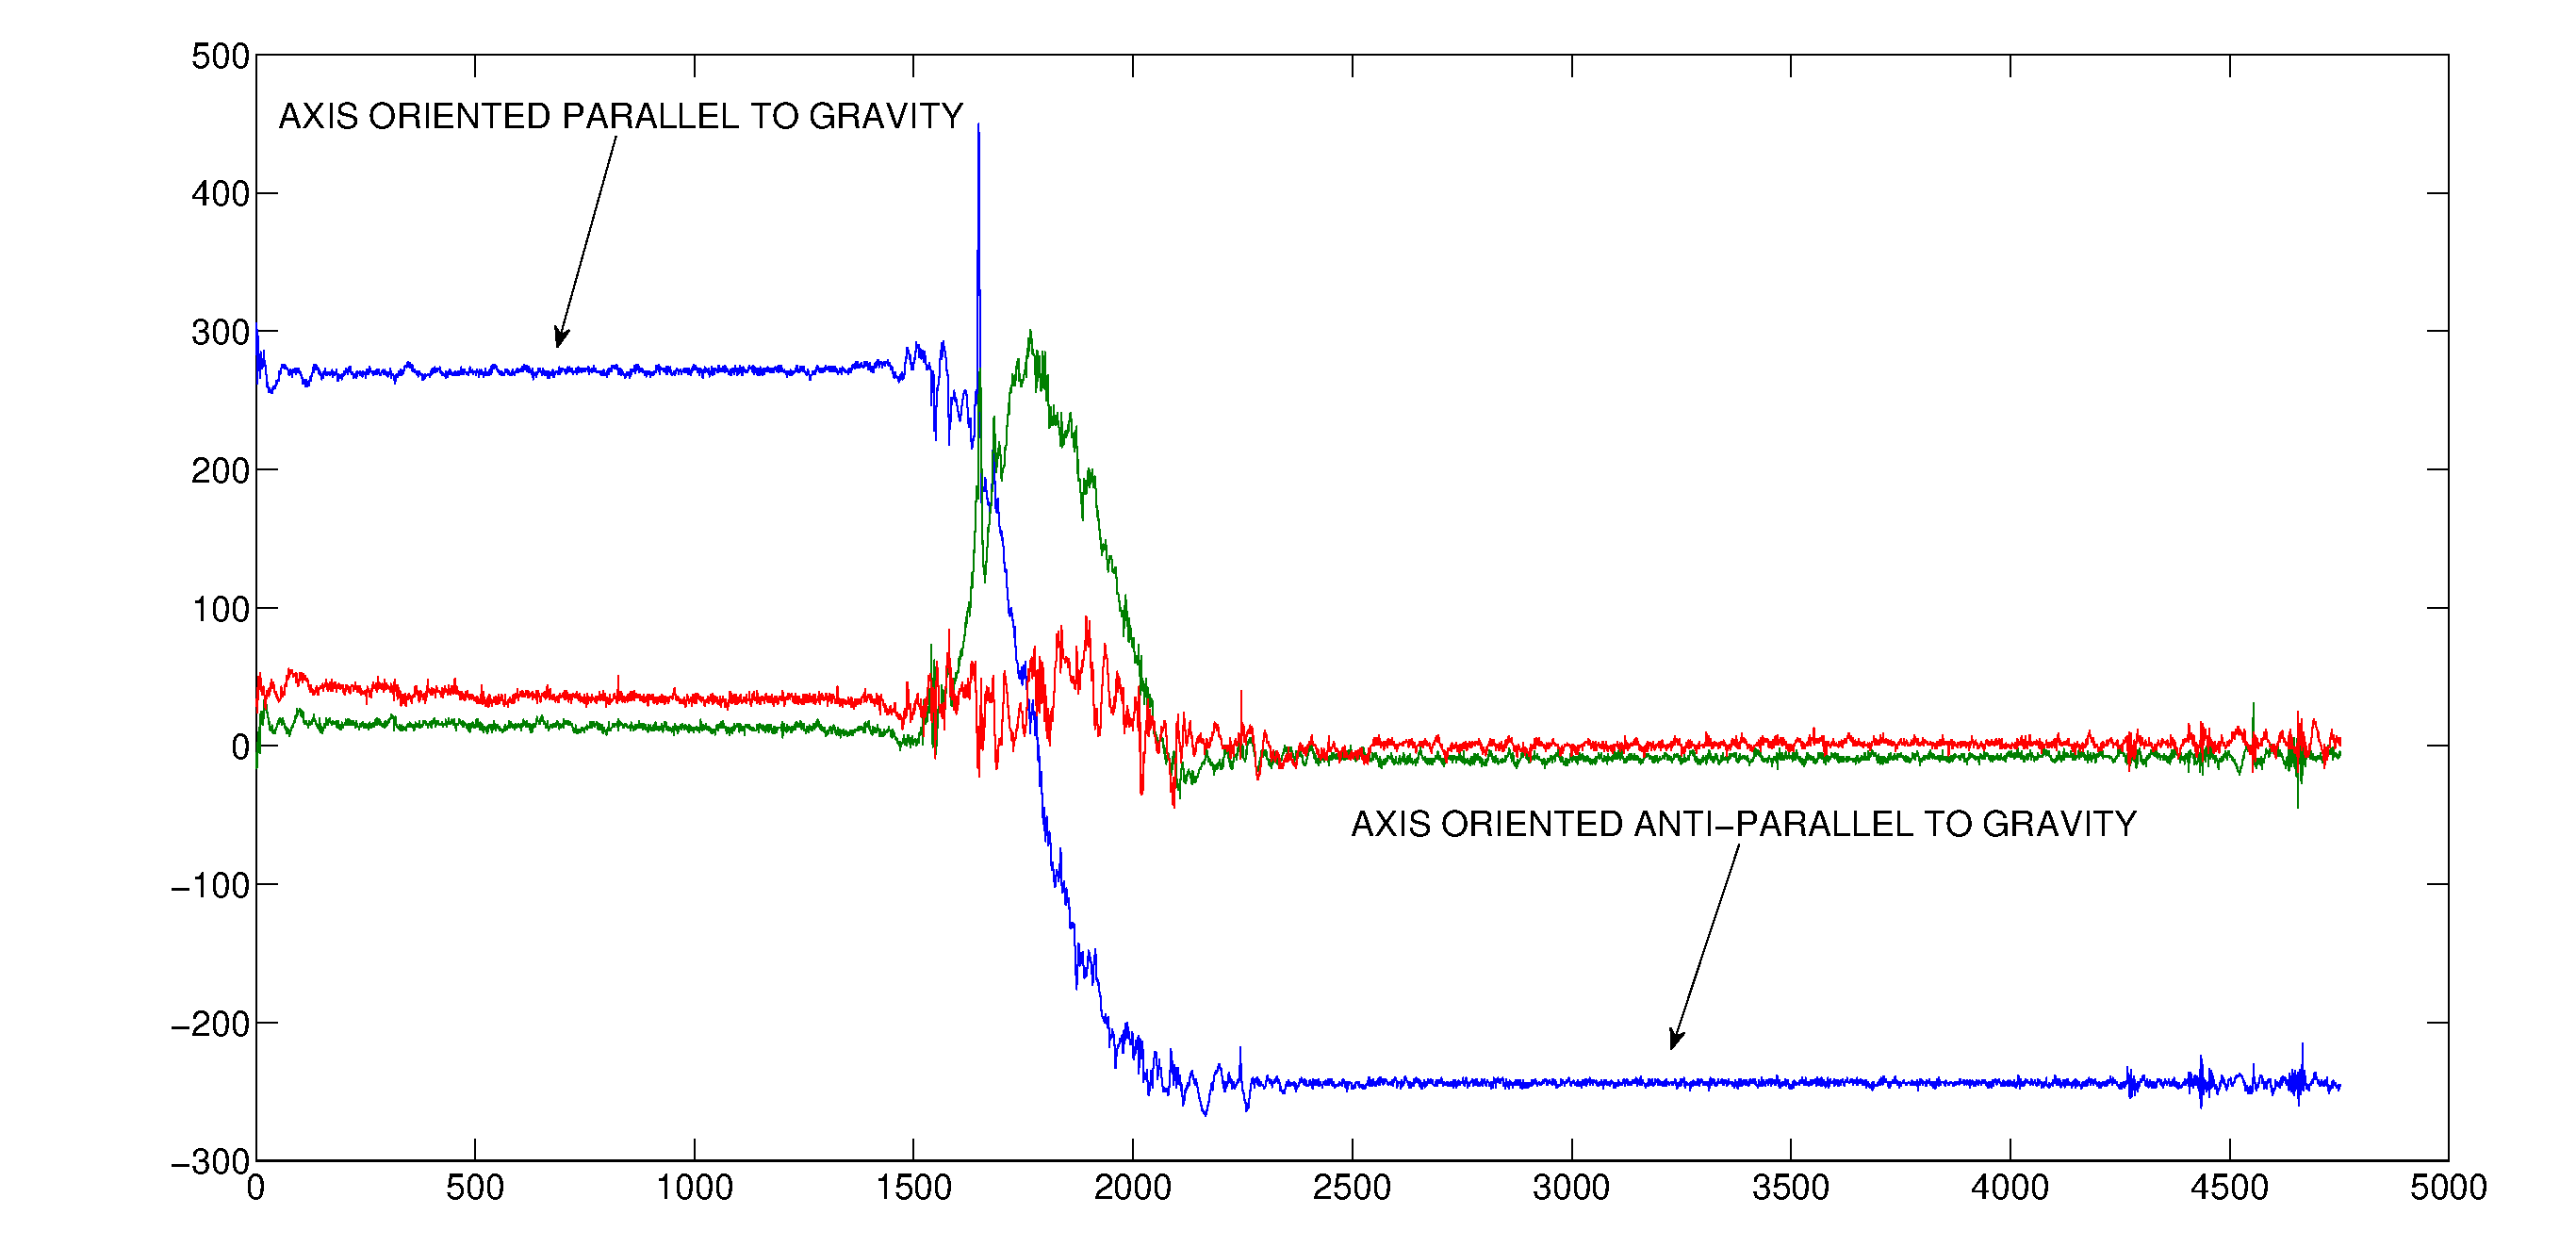
\includegraphics[width=0.85\textwidth]{figures/ZaxisAccTrunkID}
\caption{Identification of the acceleration signal gathered in the Z axis.}
\label{fig:ZaxisAccSignals}
\end{figure}

For the case of the GaitWatch, the signal showing both parallel and anti-parallel acceleration values is in channel 20. The orientation of the axis is correct, since we first put the desired Z axis pointing downwards and the accelerometer showed the largest acceleration value in that position. We, thus, set channel 20 to be the acceleration in Z axis. The remaining two axes (X and Y) are identified following the same procedure. Figure \ref{fig:XandYAccPositions} shows the box being oriented negatively and positively along X and Y axes. Both X and Y axes are properly oriented and need no orientation correction. After inspecting the gathered signals, we observe that X and Y measurements are contained in channels 22 and 21, respectively. 

\begin{figure}[H]
\centering
\includegraphics[width=0.7\textwidth]{figures/XandYAccPositions.jpg}
\caption{Identification of the box's acceleration Y (top) and X (bottom) axes.}
\label{fig:XandYAccPositions}
\end{figure}

Once we have identified the axes of the accelerometer inside the box which will be placed in the back of the patient, we need to apply the same aforementioned procedure to identify, on by one, the axes of the biaxial accelerometers which will be placed in the thighs and the shanks. Figure \ref{fig:thighShankAccs} shows the right shank module being placed parallel and anti-parallel to the gravity in both X and Z axes.

\begin{figure}[H]
\centering
\includegraphics[width=0.7\textwidth]{figures/thighShankAccs.jpg}
\caption{Identification of the Z (left) and X (right) axes of the accelerometer in right shank's unit.}
\label{fig:thighShankAccs}
\end{figure}

Table \ref{tab:acc_channels} shows the axes of all Gaitwatch's accelerometers, their associated channel and the orientation compensation (if needed).
\begin{table}
\caption{List of Gaitwatch's accelerometers and their associated channels.}
	\centering
		\begin{tabular}{|c|c|c|c|}\hline
		\label{tab:acc_channels}
		Unit 				& Axis 	& Orientation compensation 	& Channel 	\\ \hline
		Right Shank & Z			& No  (+1)									& 2					\\
		Right Shank	& X			& No  (+1)									& 3					\\
		Right Thigh & Z			& No  (+1)									& 5					\\
		Right Thigh	& X			& No  (+1)									& 6					\\
		Left Shank  & Z			& No  (+1)									& 8					\\
		Left Shank	& X			& No  (+1)									& 9					\\
		Left Thigh  & Z			& No  (+1)									& 11				\\
		Left Thigh	& X			& No  (+1)									& 12				\\
		Trunk				& Z			& No	(+1)									& 20				\\
		Trunk				& Y			& No	(+1)									& 21				\\	
		Trunk				& X			& No	(+1)									& 22				\\ \hline
		\end{tabular}
\end{table}

\subsection{Identification of Gyroscope's axes}
\label{subsec:gyro_ID}

\indent Once we have identified the axes of the accelerometers, we now proceed to identify the axes of the gyroscopes and their orientation. By convention, as it is depicted in figure \ref{fig:bodyAxes}, the sense of the rotation around a given axis is positive when the axis is pointing forwards (from the perspective of the user) and it is turned to the right. Analogously, the rotation is negative when it is turned to the left. Knowing this, in order to identify the sense of rotation of the gyroscope and adapt it (if needed) to the body frame we need to proceed as follows:
\begin{enumerate}
\item Place the axis that we want to analyze so it is pointing forwards.
\item Rotate it to the right and then to the left. Repeat this three of four times. 
\item Identify the channel containing the data and plot them. If the measured angular rate first increases and then decreases, the sense of rotation of the sensor axis is correct. On the other hand, if the angular has the opposite behavior, that is, it first decreases and then increases, we need to change the sense of the rotation. 
\end{enumerate}
Figure \ref{fig:rotation_axis_sense1} shows the maneuvers to identify the rotation sense of the Y axis gyroscope located in the left hand unit. Figure \ref{fig:rotation_axis_sense2} shows the measured angular rate for such maneuvers. Notice how the first rotation is positive (the signal increases and then decreases), so, for the case of the left hand unit, the Y axis has the correct sense of rotation.

\begin{figure}[H]
\centering
\includegraphics[width=0.7\textwidth]{figures/gyro_axis_ID.png}
\caption{Identification of the sense of rotation of the Y axis of the gyroscope in the left hand unit.}
\label{fig:rotation_axis_sense1}
\end{figure}

\begin{figure}[H]
\centering
\includegraphics[width=0.7\textwidth]{figures/gyro_axis_ID_signal.eps}
\caption{Angular rate signal gathered during maneuvers of identification of rotation.}
\label{fig:rotation_axis_sense2}
\end{figure}

This procedure needs to be repeated for each one of the axis of the gyroscopes located in all the units. \\
\indent Table \ref{tab:gyro_channels} shows the channels of all GaitWatch's gyroscopes.

\begin{table}[H]
\caption{List of Gaitwatch's gyroscopes and their associated channels.}
	\centering
		\begin{tabular}{|c|c|c|c|}\hline
		\label{tab:gyro_channels}
		Unit 				& Axis 	& Sense compensation 	& Channel 	\\ \hline
		Right shank & Y			& Yes (-1)						& 1					\\
		Right thigh & Y			& Yes (-1)						& 4					\\
		Left shank  & Y			& Yes (-1)						& 7					\\
		Left thigh  & Y			& Yes (-1)						& 10				\\
		Left arm		& Y			& No  (+1)						& 13				\\
		Left arm		& X			& Yes (-1)						& 14				\\
		Right arm		& Y			& No  (+1)						& 15				\\
		Right arm		& X			& Yes (-1)						& 16				\\
		Trunk				& Z			& No	(+1)						& 17				\\
		Trunk				& Y			& No	(+1)						& 18				\\	
		Trunk				& X			& Yes	(-1)						& 19				\\ \hline
		\end{tabular}
\end{table}

\subsection{Identification of Magnetometer's axes}
\label{subsec:mag_ID}

\indent \indent The data of the triaxial magnetometer embedded in the trunk unit are all contained in the same channel (channel 23). Each axis data has a different offset so it is easy to separate them. The axes offsets are +32764, 20000 and 0. Once we have separated the data, we need to identify which axis corresponds to each offset. To do so, we place the desired axis pointing upwards or downwards and turn the box more than 360 degrees. Then, the signal corresponding to the selected axis should be the one showing the least variation (as it is shown in figure \ref{fig:mag_axis_ID}). This operation needs to be repeated two more times to identify the remaining two axes. 
\begin{table}[H]
\caption{Magnetometer's offsets and axes.}
	\centering
		\begin{tabular}{|c|c|c|}\hline
		\label{tab:mag_offsets}
		Unit		& Axis 	& Offset 	\\ \hline
		Trunk		& X			& -20000				\\ 
		Trunk		& Y			& 0	\\ 
		Trunk		& Z			& +32764	\\ \hline
		\end{tabular}
\end{table}

\begin{figure}[H]
\centering
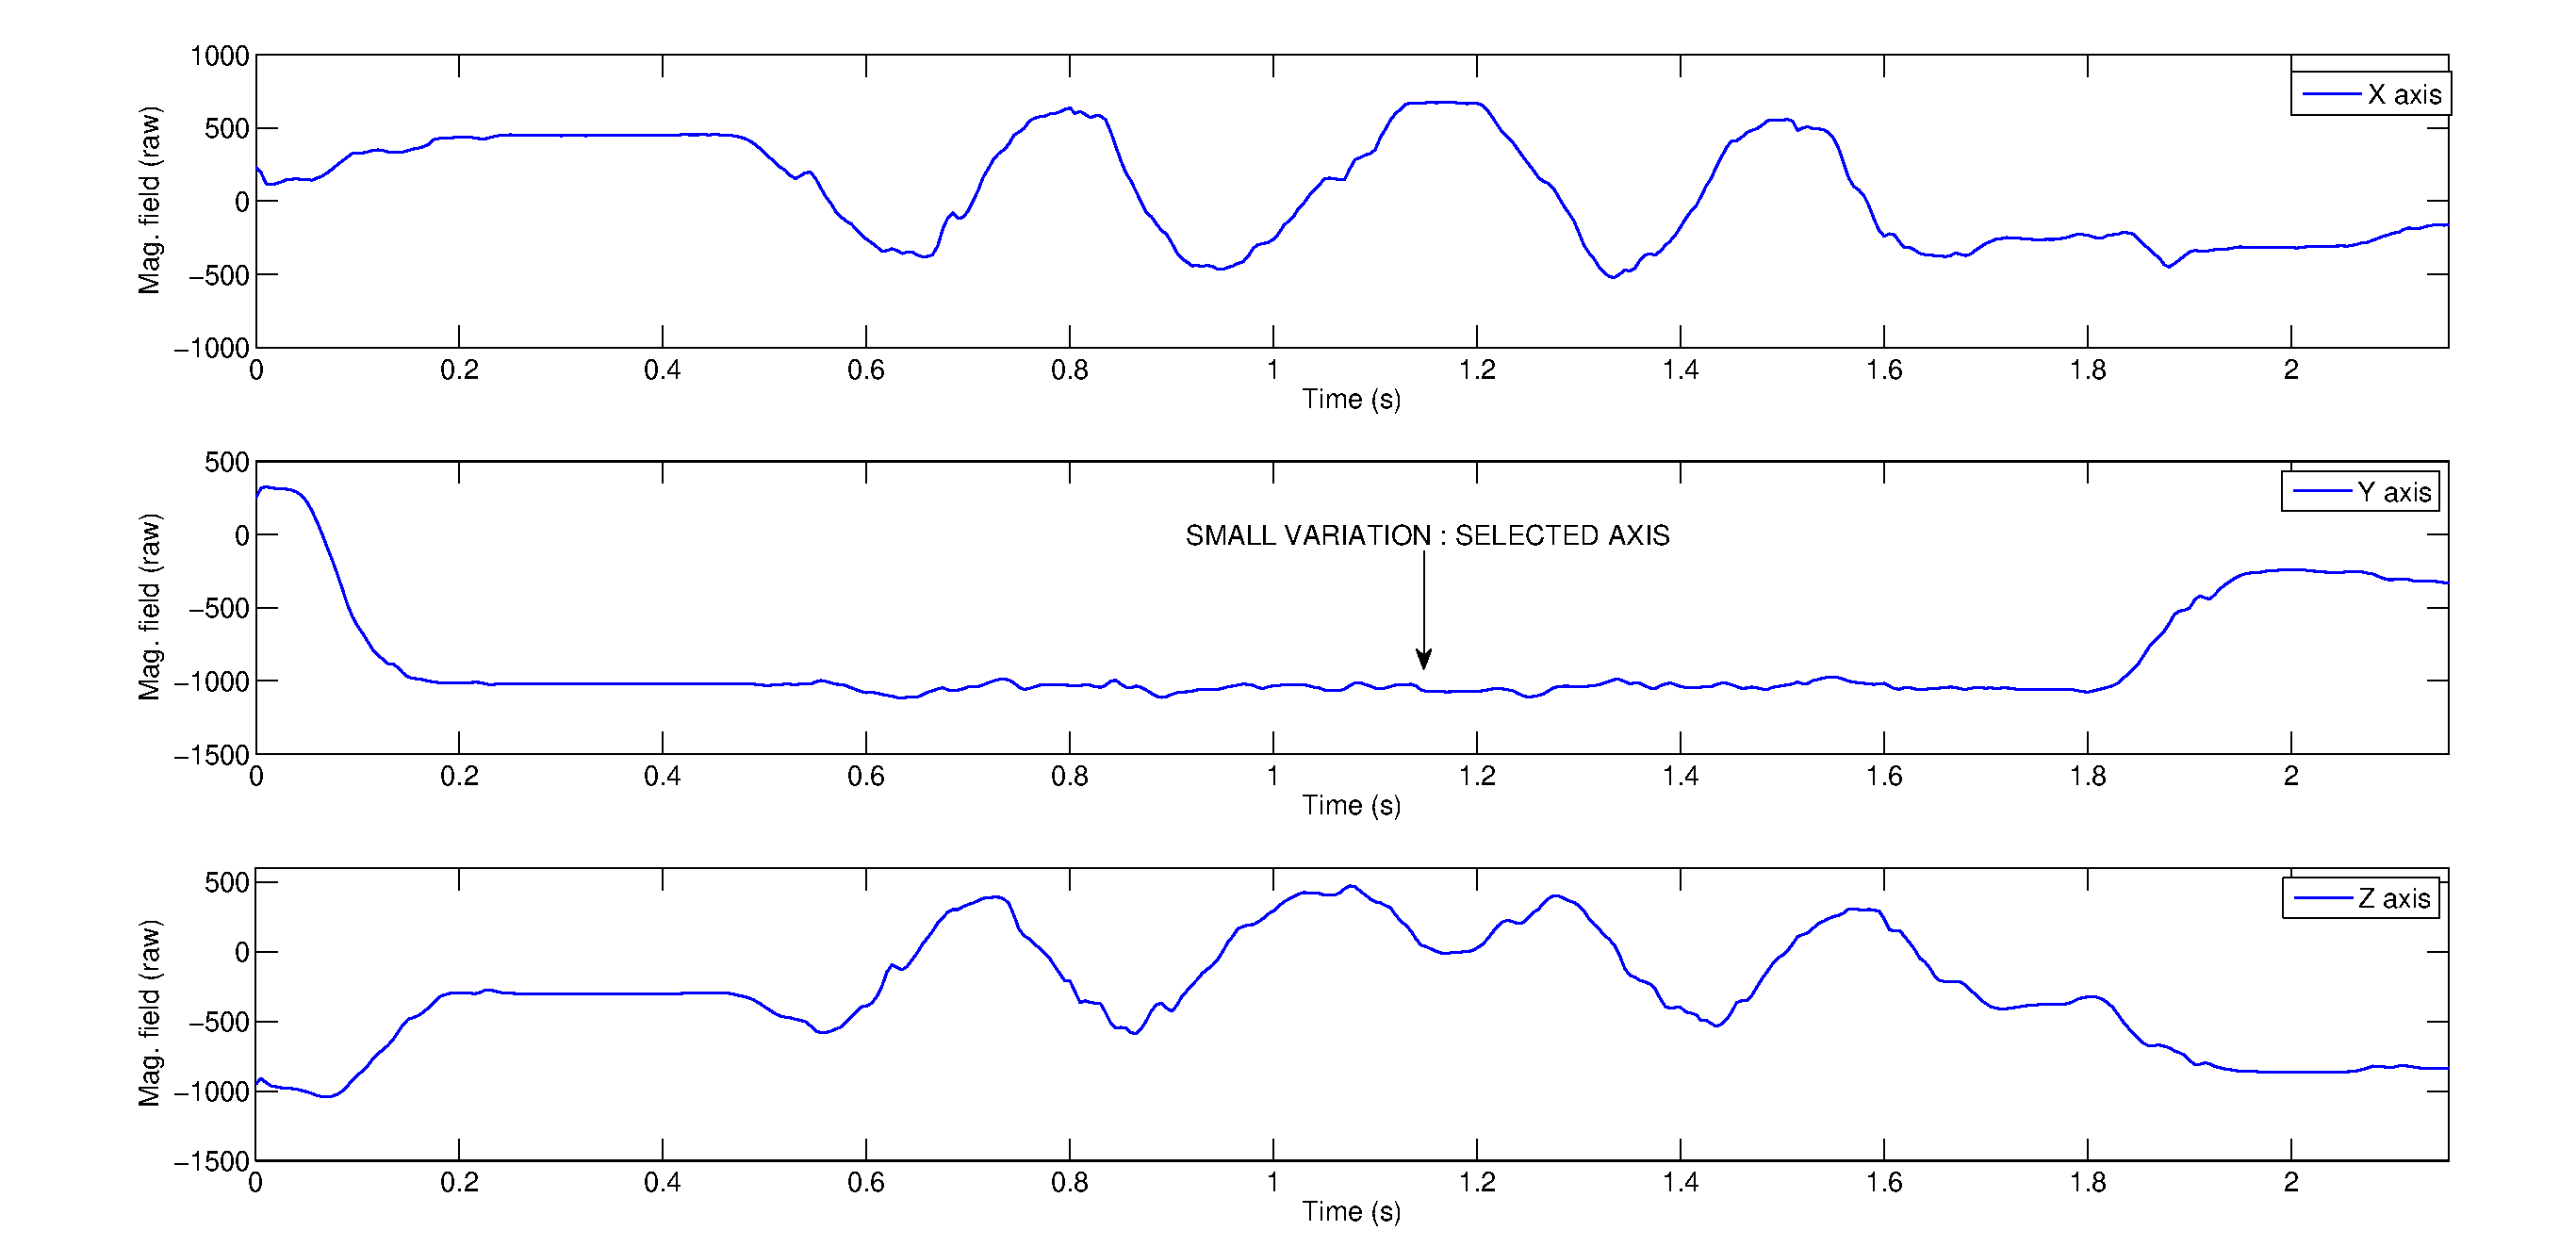
\includegraphics[width=1\textwidth]{figures/mag_axis_ID.eps}
\caption{Magnetic field signal gathered during maneuvers of Z axis identification.}
\label{fig:mag_axis_ID}
\end{figure}

